% DPF 09 talk on strangeness in nucleon

\documentclass[10pt]{beamer}
\usefonttheme{professionalfonts} % using non standard fonts for beamer
\usefonttheme{serif} % default family is serif
\usepackage{amsmath}
\usepackage{ulem}
\usepackage{hyperref}
\usepackage{array}
\usepackage{mathtools}
%\documentclass[12pt]{beamerthemeSam.sty}
\usepackage{epsf}
%\usepackage{pstricks}
%\usepackage[orientation=portrait,size=A4]{beamerposter}
\geometry{paperwidth=160mm,paperheight=120mm}
%DT favorite definitions
\def\LL{\left\langle}	% left angle bracket
\def\RR{\right\rangle}	% right angle bracket
\def\LP{\left(}		% left parenthesis
\def\RP{\right)}	% right parenthesis
\def\LB{\left\{}	% left curly bracket
\def\RB{\right\}}	% right curly bracket
\def\PAR#1#2{ {{\partial #1}\over{\partial #2}} }
\def\PARTWO#1#2{ {{\partial^2 #1}\over{\partial #2}^2} }
\def\PARTWOMIX#1#2#3{ {{\partial^2 #1}\over{\partial #2 \partial #3}} }

\def\rightpartial{{\overrightarrow\partial}}
\def\leftpartial{{\overleftarrow\partial}}
\def\diffpartial{\buildrel\leftrightarrow\over\partial}

\def\BI{\begin{itemize}}
\def\EI{\end{itemize}}
\def\BE{\begin{displaymath}}
\def\EE{\end{displaymath}}
\def\BEA{\begin{eqnarray*}}
\def\EEA{\end{eqnarray*}}
\def\BNEA{\begin{eqnarray}}
\def\ENEA{\end{eqnarray}}
\def\EL{\nonumber\\}
\def\BS{\bigskip}
\def\BC{\begin{center}}
\def\EC{\end{center}}
\def\BCC{\begin{columns}}
\def\ECC{\end{columns}}
\def\HC{\column{0.5\textwidth}}

\newcommand{\etal}{{\it et al.}}
\newcommand{\gbeta}{6/g^2}
\newcommand{\la}[1]{\label{#1}}
\newcommand{\ie}{{\em i.e.\ }}
\newcommand{\eg}{{\em e.\,g.\ }}
\newcommand{\cf}{cf.\ }
\newcommand{\etc}{etc.\ }
\newcommand{\atantwo}{{\rm atan2}}
\newcommand{\Tr}{{\rm Tr}}
\newcommand{\dt}{\Delta t}
\newcommand{\op}{{\cal O}}
\newcommand{\msbar}{{\overline{\rm MS}}}
\def\chpt{\raise0.4ex\hbox{$\chi$}PT}
\def\schpt{S\raise0.4ex\hbox{$\chi$}PT}
\def\MeV{{\rm Me\!V}}
\def\GeV{{\rm Ge\!V}}

%AB: my color definitions
%\definecolor{mygarnet}{rgb}{0.445,0.184,0.215}
%\definecolor{mygold}{rgb}{0.848,0.848,0.098}
%\definecolor{myg2g}{rgb}{0.647,0.316,0.157}
\definecolor{abtitlecolor}{rgb}{0.0,0.255,0.494}
\definecolor{absecondarycolor}{rgb}{0.0,0.416,0.804}
\definecolor{abprimarycolor}{rgb}{1.0,0.686,0.0}
\definecolor{Red}           {cmyk}{0,1,1,0}
\definecolor{Grey}           {cmyk}{.7,.7,.7,0}
\definecolor{Lg}           {cmyk}{.4,.4,.4,0}
\definecolor{Blue}          {cmyk}{1,1,0,0}
\definecolor{Green}         {cmyk}{1,0,1,0}
\definecolor{Brown}         {cmyk}{0,0.81,1,0.60}
\definecolor{Black}         {cmyk}{0,0,0,1}
\definecolor{A}{rgb}{0.8,0.0,0.0}
\definecolor{B}{rgb}{0.0,0.6,0.0}
\definecolor{C}{rgb}{0.6,0.6,0.0}
\definecolor{D}{rgb}{0.0,0.0,0.5}
\definecolor{E}{rgb}{0.4,0.4,0.4}


\usetheme{Madrid}


%AB: redefinition of beamer colors
%\setbeamercolor{palette tertiary}{fg=white,bg=mygarnet}
%\setbeamercolor{palette secondary}{fg=white,bg=myg2g}
%\setbeamercolor{palette primary}{fg=black,bg=mygold}
\setbeamercolor{title}{fg=abtitlecolor}
\setbeamercolor{frametitle}{fg=abtitlecolor}
\setbeamercolor{palette tertiary}{fg=white,bg=abtitlecolor}
\setbeamercolor{palette secondary}{fg=white,bg=absecondarycolor}
\setbeamercolor{palette primary}{fg=black,bg=abprimarycolor}
\setbeamercolor{structure}{fg=abtitlecolor}

\setbeamerfont{section in toc}{series=\bfseries}

%AB: remove navigation icons
\beamertemplatenavigationsymbolsempty
\title{
  \textbf {Introduction}\\
%\centerline{}
%\centering
%\vspace{-0.0in}
%\includegraphics[width=0.3\textwidth]{propvalues_0093.pdf}
%\vspace{-0.3in}\\
%\label{intrograph}
}

\author[W. Freeman] {Physics 211\\Syracuse University, Physics 211 Spring 2017\\Walter Freeman}

\date{\today}

\begin{document}

\frame{\titlepage}

\frame{\frametitle{\textbf{Announcements}}
\large
\BI
\item Homework 3 due tomorrow
\item Homework 4 posted; due next Friday
\item Extra office hours today, 4-7PM, in Room 208 (intended for homework help)
\item Recording of solutions to HW3: tomorrow, room 208, from 4-6PM
\pause
\BI
\item Yes, I know this is before the end of recitations
\item If you come and haven't gone to recitation yet, please turn in your homework when you arrive, and I'll get it
to your TA
\EI
\EI
}

\frame{\frametitle{\textbf{Ask a physicist: quantum computing}}
\Large

We could ask a physicist... but why not ask a politician instead?

\pause

\url{https://www.youtube.com/watch?v=Eak_ogYMprk}

\pause

\bigskip

He's mostly right: ordinary computers can explore only one possibility at a time
(per core), while quantum computers can explore many.

\bigskip\pause

... like all of the possible encryption keys for a code at once...
}

\frame{\frametitle{\textbf{Some feedback from you all}}

\large

``...swimming in a sea of applications of concepts, [without] an idea of what that overarching concept is.'' --feedback to a recitation TA, passed on to me

\pause \bigskip
The overarching concept:

\BI
\item Newton's second law $\sum \vec F = m\vec a$ tells us the relation between the forces on an object and how it moves
\item If we know the forces on an object, we can use those to compute its acceleration
\BI
\item Once we find its acceleration, we can learn about its movement, using kinematics
\EI
\item If we know its acceleration, we can go the other way, and learn about the
forces that act on it
\EI
}

\frame{\frametitle{\textbf{Breaking these bits down}}

Everything we're dealing with here is a {\color{Red}vector}:
\BI
\item Decompose all forces into $x-$ and $y-$components
\item Newton's second law becomes $(F_x = ma_x, F_y = ma_y)$
\EI
\pause
Knowing about the forces on objects:
\BI
\item Newton's {\it third} law tells us that forces come in pairs: $\vec F_{ab} = -\vec F_{ba}$
\item Normal forces are however big they need to be to stop objects from moving through each other
\item Tension is the same at all points in a rope
\item You'll learn about friction in a moment
\EI
\pause

}

\frame{\frametitle{\textbf{Breaking these bits down}}

Keeping the forces straight:

\BI
\item Draw a force diagram: a dot representing each object, with arrows going outward for each force
\item You're going to need to break forces not aligned with the (x,y) axes into components
\item Draw your diagram big enough to do the trigonometry
\EI
\pause
Applying this to Newton's second law:
\BI
\item You can look at your diagrams and read off the $x-$ and $y-$components of
the forces that are present
\item This will let you write down things like

\begin{align*}
{\textrm list\,of\,forces\,in\,x\,} =& ma_x\\
{\textrm list\,of\,forces\,in\,y\,} =& ma_y
\end{align*}

\item Do this separately for each object
\item This will give you a bunch of equations
\item Solve the system of equations by substitution for whatever you want
\EI
}

\frame{\frametitle{\textbf{A problem-solving recipe}}
  \large
\BI
\item{{\color{Red}Accounting:} Draw force diagrams for every object}
  \BI
\item{Work out components (trigonometry) of vectors in funny directions -- no need for numbers yet}
  \EI
  \pause
\item{{\color{Red}Physics:} Write down $\sum F = ma$ in each dimension, for each object}
\BI
\item Write down any constraints you have: are the accelerations of two objects related?
\item Are two forces the same magnitude by Newton's third law?
\EI
  \pause
\item{{\color{Red}Math:} Put in the stuff you know, solve for the stuff you don't}
  \pause
\item{{\color{Red}Kinematics:} Connect acceleration to motion}
  \EI
\pause

\bigskip
\bigskip

\centerline{It really is this easy; I promise!}
\pause
\centerline{``Ask physics the question, don't tell it the answer''}

}



 \frame{\frametitle{\textbf{Sample question (11:00)}}
    \Large

    A stone hangs from the roof of a car by a string; the car accelerates forward at 3 $\rm m/\rm s^2$.

    \BI
  \item{What happens to the string?}
    \pause
  \item{What angle does the string make with the vertical?}
    \pause
  \item{What is the tension in the string?}
    \EI
  }

\frame{\frametitle{\textbf{Sample question (9:30)}}
\Large

Two weights, of mass $M$ and $m$, hang from a light, frictionless pulley. How do they move when they are released?

}

\frame{\frametitle{\textbf{Sample questions}}
    \Large

    A cart slides down a frictionless track elevated at angle $\theta$; what is its acceleration?

}

\frame{\frametitle{\textbf{A new force: Friction}}
  \large
  \BI
\item{Friction: stops two surfaces from sliding past each other}
\item{Can either make things move or make things stop; opposes {\it relative} motion}
\item{Two types:}
\BI
\normalsize
\item{Static friction: keeps two things that aren't sliding stuck together}
\item{Kinetic friction: opposes the relative motion of two things sliding}
\EI
\EI
\bigskip
\bigskip
}

\frame{\frametitle{\textbf{Coulomb's friction model}}
  \large
  \centerline{\bf Friction is really complicated!}
  \BI
\item{Depends on details of surfaces, molecular forces, etc.}
\item{No way to create a completely accurate general principle}
  \EI

  \bigskip
  \bigskip

  \centerline{\bf There are a few general principles, though:}
  \BI
\item{Friction is higher if the normal force is higher}
\item{Kinetic friction doesn't depend that much on the speed of travel}
  \EI

  \bigskip
  \bigskip

  \centerline{\bf Simple model: often pretty close}
  \BI
\item{Friction depends on a property of the surfaces called the {\color{Red}coefficient of friction} $\mu$}
\item{Force of kinetic friction = $\mu_k F_N$}
\item{Max force of static friction = $\mu_s F_N$}
  \EI
}

\frame{\frametitle{\textbf{Friction, a summary}}
\large
\BI
\item Kinetic friction points in whichever direction opposes the relative motion
\item $F_{f,k} = \mu_k F_N$
\EI
\bigskip
\bigskip
\BI
\item Static friction points in whichever direction it needs to in order to keep the objects from sliding
\item You will need to think carefully about this: the direction can change, 
depending on other things
\item Static friction is however big it needs to be to keep the objects from sliding, up to a maximum value:
\item $F_{f,s,\rm max} = \mu_s F_N$
\EI
}

\frame{\frametitle{\textbf{Traction}}
Wheeled vehicles use friction between their wheels and the ground 
to accelerate themselves.

\bigskip

We call this force ``traction''. It can point in either direction, depending on how
the car is trying to turn its wheels, with the engine, brakes, or so on.

\bigskip
\pause
In normal use, though, the piece of the wheel touching the ground does not move.

\bigskip
This means that the traction force is really {\color{Red}\bf static friction}.

So $$F_{\rm trac} < \mu_s F_N,$$ just like for static friction. It points
either forwards or backwards, depending on what the engine/brakes/bicyclist/etc.
are doing.
} 


\frame{\frametitle{\textbf{Coefficients of friction}}

  \centerline { 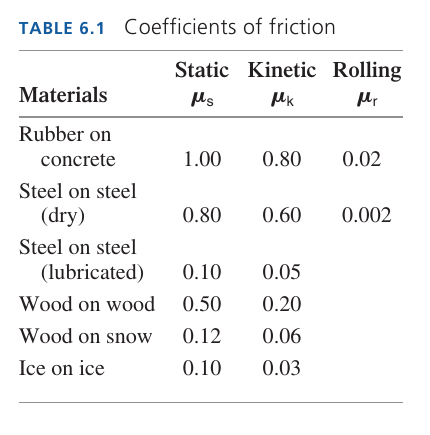
\includegraphics[width=0.5\textwidth]{mu-table.png}}
}

 \frame{\frametitle{\textbf{Sample questions}}
    \Large

    A block slides down a track elevated at angle $\theta$ with $\mu_k$ known; what is its acceleration?
  }

\frame{\frametitle{\textbf{Sample questions}}
    \Large
  A block with mass $m$ on a track is connected by a rope to a hanging weight of mass $M$. The coefficients of friction are $\mu_s$ and $\mu_k$. What is the acceleration of both objects?

  }






\end{document}
